\documentclass{article}
\usepackage{graphicx} % Required for inserting images
\usepackage[
% backend=biber,
style=alphabetic, % alphabetic, numeric
natbib=true,
% maxnames=1,
% sorting=ynt
]{biblatex}
\AtEveryBibitem{
    \clearfield{urlyear}
    \clearfield{urlmonth}
}
\usepackage{hyperref}
\usepackage{xcolor}
\usepackage{amssymb}
\usepackage{amsmath}
\usepackage{wrapfig}
\usepackage{multirow}  % tables double entry
\usepackage{geometry}
\usepackage{bbm}  % makes mathbbm{1} vector 1
\usepackage{cleveref}
\usepackage{algorithm}
\usepackage{algpseudocode}
\usepackage{parskip}
\usepackage{amsthm}
% tables
\usepackage{booktabs}
\usepackage{tabularx} % For text wrapping in the last column
\usepackage{multirow} % Required to span cells across rows

% for definitions
\theoremstyle{definition}
\newtheorem{definition}{Definition}[section]
\newtheorem{example}{Example}[section]
\theoremstyle{remark}
\newtheorem*{remark}{Remark}
\newtheoremstyle{resultstyle}% name of the style to be used
  {10pt}% measure of space to leave above the theorem. E.g.: 3pt
  {\topsep}% measure of space to leave below the theorem. E.g.: 3pt
  {\itshape}% name of font to use in the body of the theorem
  {0pt}% measure of space to indent
  {\bfseries}% name of head font
  {. ---}% punctuation between head and body
  { }% space after theorem head; " " = normal interword space
  {\thmname{#1}\thmnumber{ #2}\textnormal{\thmnote{ (#3)}}}
\theoremstyle{resultstyle}
\newtheorem{theorem}{Theorem}[section]
\newtheorem{proposition}{Proposition}[section]
\newtheorem{conjecture}{Conjecture}[section]
\newtheorem{corollary}{Corollary}[section]
\newtheorem{lemma}{Lemma}[section]

\geometry{margin=1in}
% \setlength\parindent{10pt}  % Paragraph indentation
\newcommand{\pnote}[1]{\textcolor{red}{PL: #1}}
\newcommand{\myline}{%
  \vspace{5mm}%
  \hrule%
  \vspace{5mm}%
}

\addbibresource{references.bib} %Import the bibliography file

\title{Symmetries and Deep Learning: a Survey}
\author{Pierrick Leroy}
\date{2026}

\begin{document}

\maketitle

\begin{abstract}
% Audience: reader curious to know about occurences of symmetries in a deep learning context

\pnote{write at the end}

\end{abstract}

\section{Introduction}

\pnote{write at the end}

% First paragraph of the introduction in ennes2025fcm

\subsection{Methodology}
% Starting point: initial stack of paper collected over 2 years along the way
% Completion of the initial stack by keyword search on scopus, google scholar and by AI powered tools like research-rabbit or elicit
% Criterion for retaining a reference: published in a peer-reviewed venue OR high impact (>100 citations on google scholar) OR recent (publication date<2 years)

% The different sections have some degree of overlap and the positioning of branches in the taxonomy is indicative of main tendencies but not capturing all the diversity or granularity (many works combine different technique, or could be classified in two different ways depending on what is put forward). It is a simplifying picture.

\subsection{Related work}
We list previous work that have collected or formalized literature on symmetries in a deep learning context.
Symmetric architecture (such as Siamese networks) are surveyed in \cite{ilina2022sa}.
\cite{zhao2025} focuses on parameter-space symmetries: transformation that change the representation of a neural network but do not modify the implemented function.
\cite{sipiran202523scgpis} references symmetry discovery methods in 3D shapes
% geometric deep learning
\cite{bronstein2021} is the reference textbook on geometric deep learning,  \cite{gerken2021,carlsson} study the mathematical formalism of this field and \cite{basheer2025ijdsa,habte2023} focus more specifically on equivariant convolutions, \cite{fei2024air} on 3D rotations and \cite{seo2025a} on robotics.
\cite{rath2024air} gathers methods that integrate geometric prior knowledge to neural network such that their representations are invariant or equivariant.


\section{Background}

% Conservation laws ?

\subsection{What is a Symmetry?}



A \textit{symmetry} is a transformation that leaves an object as a whole unchanged, it is statement about identity.
\textit{Invariance} is a broader, functional term that refers to the situation where a property of an object does not change under a transformation.
Symmetry can be defined by invariance by saying that an object has a symmetry if its identity is invariant under a specific transformation.

\begin{definition}[$\phi$-equivalence, {\cite{cohen2014}}]\label{def:equivalence}
    Let $\phi : \mathcal{X} \to \mathcal{Y}$ be a function from an input domain $\mathcal{X}$ to a codomain $\mathcal{Y}$, where for example $\mathcal{X} \subseteq \mathbb{R}^d$, and $\mathcal{Y}$ may be $\{0,1\}$ (binary classification), $\{1,\dots,L\}$ (multiclass classification), $\mathbb{R}$ (regression), or $\mathbb{R}^e$ (feature representation).
    
    Two elements $x, y \in \mathcal{X}$ are said to be \emph{$\phi$-equivalent}, denoted $x \sim_{\phi} y$, if
    \[
        \phi(x) = \phi(y).
    \]
    The relation $\equiv_{\phi}$ is an equivalence relation on $\mathcal{X}$ and induces a partition of $\mathcal{X}$ into equivalence classes.
    \end{definition}

\begin{example}[Image segmentation]\label{ex:image-segmentation}
    If $\mathcal{X}$ is an image, $x\in \mathcal{X}$ a pixel and $\mathcal Y = \left \{ 1\dots L\right \}$ are segmentation labels, then the sets defined by the equivalence relation are the pixels that belong of the same segmentation class.
\end{example}

\begin{example}[Image classification]\label{ex:image-classification}
    If $\mathcal{X}$ is a \emph{set of images}, $x\in \mathcal{X}$ is an image, $\mathcal Y = \left \{ 1\dots L\right \}$ are the labels, then the sets defined by the equivalence relation are images of the same class.
\end{example}

\begin{example}[Loss level sets]
    If $\mathcal Y = \mathbb R$ and $\phi$ is a generic loss function, then the sets defined by the equivalence relation are the level set of the loss function.
\end{example}

\begin{example}[Observationally equivalent parameters]\label{ex:equivalence_observational}
    If $\mathcal X$ a parameter space, $\mathcal{Y}$ a functional space and $\phi$ is the implementation map then the sets given by the equivalence relation $\phi$ are the observationally equivalent parameters
\end{example}

\begin{definition}[Invariance]\label{def:invariance}
    Let $G$ be a group acting on a set $\mathcal{X}$.
    A function $\phi : \mathcal{X} \to \mathcal{Y}$ is $G$-invariant if $\phi(g\cdot x)=\phi(x)$ for all $g\in G$ and $x\in X$.
\end{definition}

In \cref{ex:image-classification,ex:image-segmentation}, $G$ acts on images and could contain translations, rotations or reflections while in \cref{ex:equivalence_observational}, $G$ acts on parameters and contains transformations that leave the implemented function unchanged such as within-layer neuron permutations for MLPs.

\begin{definition}[Equivariance]\label{def:equivariance}
    Let $G$ be a group acting on sets $\mathcal{X}$ and $\mathcal{Y}$. 
    A function $\phi : \mathcal{X} \to \mathcal{Y}$ is $G$-equivariant if
    \[
        \phi(g \cdot x) = g \cdot \phi(x)
    \]
    for all $g \in G$ and $x \in \mathcal{X}$.
\end{definition}

In equivariance, the group $G$ acts both on the input and output.
$G$ can act similarly on the two sets, as it can be the case for 3D physical data \cite{geiger2022,bogatskiy2020p3icml}, for example when studying forces acting on a molecule one might want to encode in $G$ the fact that when rotating the molecules, a similar rotation must be applied to the forces.
A similar case is in image segmentation where translation of the domain must induce the same translation of segmentation map.

However, equivariance does not require that the group $G$ acts in the same way on input and output \cite{cohen2016a,bogatskiy2020p3icml}.
Formally, let $T$ and $T'$ be two transformations taking inputs from $G$ and forming $T_g$ and $T_g'$ acting on $\mathcal{X}$ and $\mathcal{Y}$ respectively.
In general, the only requirement is that $T$ and $T'$ are linear representations of $G$, \textit{i.e.} that the following holds: 

\begin{equation}\label{eq:general-equivariance}
    T(gh)=T(g)T(h) \quad \textrm{and} \quad T'(gh)=T'(g)T'(h) \qquad \forall g, h \in G.
\end{equation}

From \Cref{eq:general-equivariance}, we see that invariance can be realized as a special case of equivariance, namely taking $T'(g)=id_{\mathcal Y}$ for all $g$.
In words, $T'$ maps all group elements to the identity group action.


\subsection{ Mathematical Foundations of Symmetry}
% Group Theory: discrete (permutation, cyclic…) or continuous/Lie (Euclidean, Lorentz) groups and Lie algebra, representation theory and irreducible representations
% Group action, Tensor algebra, spherical harmonics (used a lot in Euclidean neural networks)
% Manifold/Gauge Theory: fiber bundles, local symmetries
% Homogeneous space
% Category theory
% \cite{borde2025,carlsson,chen2020,2023tg,bronstein2021}

\subsection{Taxonomy and paper organization}
% A taxonomy where each cell contains a branch name and a few representative works
% The linear structure of the paper is organized along the methodological dimension of the taxonomy

We propose a few criterion to categorize occurrences of symmetries in a deep learning context.


\begin{table}[h]
    \centering
    \begin{tabularx}{\textwidth}{|c|c|c|c|X|}
        \hline
        \textbf{Main} & \textbf{Values} & \textbf{Secondary} & \textbf{Values} & \textbf{Description} \\
        \hline
        Exactness & Exact       &          &          & \multirow{3}{=}{Whether the symmetry exactly holds or not.} \\
                  & Approximate &          &          & \\ % Leave the last column empty here
                  & Partial &          &          & \\ % Leave the last column empty here
        \hline
        Methodology & Prescriptive & Encoding & Implicit & \multirow{3}{=}{How the researcher interacts with the symmetry. Prescriptive assumes a-priori knowledge of the symmetry.} \\
                    &              &          & Explicit & \\ % Leave the last column empty here
        \cline{2-4}
                    & Descriptive &  &  & \\
        \hline
        Object & Data & & & \multirow{4}{=}{What is the relevant scope to consider the symmetry. Data, model and framework are not mutually exclusive.} \\
        \cline{2-4}
               & Model & State & Fixed & \\
               &       &       & Dynamic & \\
        \cline{2-4}
               & Framework      &       & & \\
        \hline
    \end{tabularx}
    \caption{\textbf{Main}. Top level criterion \textbf{Secondary}. Optional second level, depending on the value of the main criterion. The main criterion are independent, the secondary level is hierarchically dependent on the main level.}
    \label{table:taxonomy}
\end{table}

% Description of the table criteria: approximate if it holds to first order but not strictly (\textit{e.g.} due to noise), incomplete for a restriction (\textit{e.g.} subset of the group
% Partial vs approximate terminology from \cite{petrache2023}

\begin{figure}
    \centering
    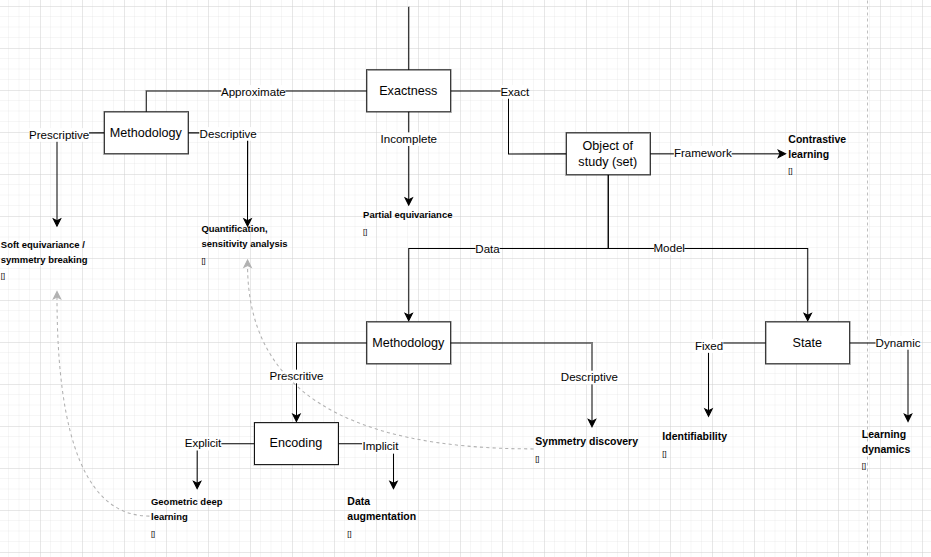
\includegraphics[width=0.75\linewidth]{images/draft/taxonomy.png}
    \caption{Classification tree based on the taxonomy from \Cref{table:taxonomy}}
    \label{fig:taxonomy}
\end{figure}


\section{Symmetry as a design principle}



\subsection{Geometric deep learning}

% Irreducible representation (seems to be particularly used for E(n) equivariance)
% add citation to dehmamy2021anips: achieve equivariance through Lie algebra

Geometric Deep Learning (GDL) \cite{bronstein2017ispm,bronstein2021} is concerned with the design of equivariant layers on various geometric domains.
It provides a unifying framework for deep learning architectures by viewing them through the lens of symmetry and group equi\slash invariance.
Its central thesis, inspired by Felix Klein's Erlangen Program, is that the appropriate inductive bias for a learning problem is determined by the symmetries of its domain.
This perspective simultaneously furnishes a common mathematical framework for existing architectures such as CNNs, RNNs, GNNs and Transformers, and a constructive blueprint for designing new ones on non-Euclidean domains such as graphs and manifolds.
As a result, equivariant neural network architectures typically benefit from fewer learnable parameters, better interpretability (\textit{e.g.} CNNs filter), robustness guarantees (since the network behavior is dictated by symmetry groups, its response to some data manipulation is deterministic) and generalization properties (out-of-distribution data points can become in-distribution once a symmetry is imposed \textit{e.g.} an image with an upside down car).
An accessible treatment of the underlying mathematical foundations is given in \cite{borde2025,gerken2021,carlsson}.

\paragraph{The role of convolution}
\cite{cohen2016} showed how convolutional networks can be generalized into Group Convolutional neural networks (G-CNNs) to exploit larger groups of symmetries, including discrete rotations and reflections.
An important result of GDL is obtained by \cite{kondor2018p3icml} for compact groups.
They provide general guidelines for constructing equivariant neural networks with respect to compact groups and show that the convolutional structure is not just sufficient but necessary for designing equivariant NN (under some hypotheses).
Similar statements are obtained in the context of the $SE(3)$ group\cite{weiler2018anips} and for homogeneous spaces in \cite{cohen2019anips} by rephrasing G-CNNs in a general fiber bundle formalism.

\paragraph{Euclidean transformations}
% Tess schmidt, Euclidean neural network, spherical harmonics, irreducible representations
An important branch of GDL is concerned with Euclidean transformation since these are pertaining to the physical world.
For planar images, \cite{weiler2019anips} provides a general description of $E(2)$-equivariant convolutions in the Steerable CNN framework \cite{cohen2016a}, constraining convolution kernels via the irreducible representations of the group, yielding a kernel basis whose elements are combined by learnable weights and thus ensuring equivariance.
Spherical CNNs \cite{cohen2018} uses a generalized Fast Fourier Transform to achieve $3$D rotation equivariance and the $SE(3)$ case is addressed in \cite{weiler2018anips}.
A practical software framework implementing $E(3)$-equivariant operations including tensor products, spherical harmonics, and attention mechanisms is provided by \texttt{e3nn} \cite{geiger2022}.

\paragraph{Extensions}
% Lie groups
\cite{finzi2020p3icml} proposes a general method to construct equivariant convolutional layers for any Lie group with a surjective exponential map.
\cite{finzi2021p3icml} provides a general algorithm for constructing equivariant MLP for arbitrary matrix groups by collecting symmetry constraints and solving the system with an SVD decomposition, recovering known solutions as special cases.
G-CNNs are further generalized to arbitrary Lie group in \cite{bekkers2021}.
% Gauge
A gauge-equivariance perspective is given by \cite{cohen2019p3icml,gerken2021,weiler2026,boyda2021prd}.

\paragraph{Permutations}
When data is unstructured (sets), spatially unorganized (point clouds), or defined on a graph, models must be invariant to the order of input elements.
\cite{zaheer2018} characterizes permutation-invariant functions on sets and derives necessary and sufficient conditions for permutation equivariance in deep models, showing that any such function decomposes into a sum of per-element transformations followed by a global aggregation (universal approximation of set functions) and \cite{lee2019p3icml} extends the methods to allow for interaction between set elements with an attention-based architecture.
PointNet \cite{qi2017a} pioneered deep learning directly on raw point clouds by applying a symmetric aggregation function to independently transformed elements, and PointNet++ \cite{qi2017} introduced hierarchical local grouping to capture multi-scale geometric structure.
\cite{wang2019} bridges point clouds and graphs by dynamically computing a k-nearest-neighbor graph in feature space at each layer, enabling richer local context without a fixed input graph.

On graphs, permutation equivariance applies to the node indices.
The message passing framework \cite{gilmer2017} unified earlier graph models \cite{duvenaud2015,kipf2017,bruna2014} into a single formalism involving a message function, an aggregation function (enforcing permutation invariance), and an update function.
\cite{velickovic2018} incorporated an attention-like mechanism into this scheme while preserving permutation invariance.
% TODO: morris2019pacai, xu2019, bouritsas2021, bodnar2021a, maron2020

For geometric graphs, where nodes carry coordinates in $\mathbb{R}^3$, permutation equivariance must be combined with Euclidean symmetries.
\cite{satorras2021p3icml} achieves joint $E(n)$-equivariance and permutation equivariance through invariant edge features based on interpoint distances, without requiring costly higher-order representations.
\cite{fuchs2020} attains $SE(3)$-equivariance via self-attention on steerable features, at higher computational cost but with greater expressivity.

\paragraph{Applications}
GDL principles have been successfully applied to a wide range of domains. In molecular science, \cite{satorras2021p3icml} demonstrates joint $E(n)$-equivariance and permutation equivariance for chemical property prediction and $n$-body dynamics, while \cite{cornet2024} extends this to equivariant diffusion models for 3D molecule generation.
Atomic energy and force prediction benefit from equivariant graph transformers such as Equiformer \cite{liao2022} and its scaled variant EquiformerV2 \cite{liao2023}.
In structural biology, AlphaFold \cite{jumper2021na} and RoseTTAFold \cite{baek2021s} leverage geometric inductive biases for highly accurate protein structure prediction, while \cite{townshend2021s} applies $SE(3)$-equivariant networks to RNA structure scoring, achieving state-of-the-art results in a limited data settings.
In particle physics, \cite{bogatskiy2020p3icml} introduces Lorentz-group equivariant networks for jet classification, obtaining competitive performance with substantially fewer parameters than non-equivariant baselines.
In medical imaging, \cite{winkels2019mia} shows that 3D G-CNNs significantly improve pulmonary nodule detection in CT scans over standard convolutional counterparts again in a low data regime.
In natural language processing, \cite{gordon2020} exploits permutation equivariance to explore compositional generalisation.
In computer vision, equivariant networks have been applied to omnidirectional images and global climate pattern recognition via spherical CNNs \cite{cohen2018,cohen2019p3icml}, and to 3D object detection \cite{yu2022}.
For robotics and 3D scene understanding, equivariance to Euclidean transformations is a natural requirement, as surveyed in \cite{seo2025a,fei2024air}.

\paragraph{Expressivity}
% Expressivity: do symmetry constraints impact the approximation power of GDL models ?
Enforcing symmetry constraints raises the question of expressivity (or \textit{universality} \cite{maass2024}) \textit{i.e.} the ability to represent an arbitrary function within its symmetric hypothesis class.
In that regard, distinguishing non-isomorphic graphs has been a central theoretical concern in the GNN community: \cite{xu2019} proved that message passing networks are at most as powerful as the Weisfeiler--Lehman (WL) graph isomorphism test, and \cite{maron2020} showed that higher-order tensor networks can match higher-order WL tests.
Subsequent work sought to surpass the 1-WL barrier by incorporating structural features: \cite{bouritsas2021} counts subgraph isomorphisms, and \cite{bodnar2021a} lifts graphs to cell complexes, achieving provably greater expressivity while retaining efficient computation.
Universality results remain scarce, for Euclidean equivariant networks \cite{yarotsky2018r} establishes universal approximation for invariant maps, and \cite{bogatskiy2020p3icml} proves universality for Lorentz-equivariant models, while \cite{kondor2018p3icml} shows that equivariant linear maps between feature spaces over homogeneous spaces are necessarily generalized convolutions and \cite{pacini2026} establishes that shallow equivariant models can fail to be universal, but that sufficient depth or the addition of appropriate readout layers restores universality within the entry-wise separable regime.

\paragraph{Optimization challenge}
% Optimization of GDL models: does the symmetry constraint make optimization harder compared to a vanilla model ?
Maintaining exact equivariance can introduce significant computational overhead.
Models based on irreducible representations are computationally heavy even though recent work has optimized the tensor product decomposition \cite{passaro2023,luo2024a}.
Equivariant architectures may require higher numerical precision, larger memory footprints, longer wall-clock training times relative to unconstrained counterparts and have a dependence to the input size which can limit their scalability to large systems \cite{bogatskiy2020p3icml}.
Optimization difficulties for equivariant neural networks have been observed \citep{pertigkiozoglou2024,lawrence2026}.

\paragraph{Equivariant or vanilla architectures ?}
% Equivariant architecture vs vanilla
A practical question is whether the design costs, potential difficulties in optimization and hardware regret due to less mature technology of equivariant models is justified over a simpler model, possibly trained with data augmentation.
\cite{nordenfors2024} compare stability of equivariant and vanilla counterpart with data augmentation and \cite{shen2026} provides empirical evidence that, for 3D-rotation equivariant tasks, unconstrained models trained with augmentation reduce their equivariance error rapidly to below 2\% of the total loss within thousands of steps
However equivariant architectures are arguably preferable when data is scarce, when physical consistency of predictions is required, or when generalization to unseen orientations or configurations is critical.
\citet{lawrence2026} propose a decision rule depending on the amount of symmetry bias in the dataset and its correlation with labels.
On the theoretical side, \cite{elesedy2021p3icml} obtain a strict generalization benefit in favor of equivariance for linear models.

\paragraph{Real-world applicability}
% Which problems remain challenging
Many real-world datasets only approximately satisfy a given symmetry, for instance due to sensor noise, occlusions, or genuine symmetry breaking in the underlying phenomenon and in that case strictly equivariant models may then be over-constrained (see other sections).

\subsection{Data augmentation}
Data augmentation (DA) enriches a training set by applying transformations that are known, or assumed, to leave the target label unchanged.
Formally letting $G$ act on input space $\mathcal X$, the augmented risk replaces the standard empirical risk by averaging over orbits:
$$
\hat R_{\text{aug}}(\theta)=\frac{1}{|G|}\sum_{g\in G}\hat R(\theta |g\cdot \mathcal D),
$$
with the hope of encouraging the learned function to be approximately invariant to those transformations (for a continuous group, an expectation is taken over a distribution on $G$).
Compared to designing an equivariant architecture, DA is attractive in several practical scenarios: it can be applied on top of any pretrained model without architectural changes, making it well-suited to fine-tuning; it requires no group-theoretic implementation, lowering the barrier for rapid prototyping; it naturally accommodates complex or poorly characterized transformations (\textit{e.g.} variations in illumination, viewpoint, or background in images) not easily amenable to an algebraic description and it handles approximate or partial symmetries without additional formalism.
On the downside, covering a continuous symmetry group is impossible and materialized augmentation increase storage and compute requirements proportionally to the number of samples drawn per group orbit.

\paragraph{Theoretical approaches}
\citet{chen2020} propose a group theoretical framework for s and formally connects orbit averaging with lower generalization error.
Variance reduction results can also be obtained \citep{chen2020,dao2019p3icml}.
The notion of orbit averaging is declined and practically implemented in \citet{benton2020anips}.
For infinite width and kernel classifier settings,  is shown to be equivalent to symmetrization of the model \citep{maass2024,dao2019p3icml}.
\citet{lyle2020} extend PAC-Bayes bound to DA and obtain variance reduction for the empirical risk.
The value of DA might be context dependent with relevant aspect being the learning regime (over- or underparametrized) and task (classification or regression).
A spectral point of view is given in \citet{lin2024} while \citet{lawrence2026} further studies the role of the symmetry distribution.

\paragraph{Automated  strategies}
Rather than hand-crafting augmentation policies, several works have proposed to search for them automatically.
\citet{cubuk20192iccvprc} introduce AutoAugment, which uses reinforcement learning to find a policy composed of image-processing operations such as rotations, translations, and shearing, optimized for validation accuracy.
\citet{lim2019anips} reduced the search time by leveraging Bayesian optimization over policies and using \textit{density matching} as a criterion: a minimization of the divergence between the augmented and training distributions and a differentiable approach was proposed in \citet{hataya2020cv-e2} by training a generative adversarial network (GAN) to output augmentation parameters minimizing a similar density-matching objective, further accelerating the search.
Another strategy is to transfer augmentations across domains: \citet{antoniou2018} learn a GAN on a data-rich source domain and replay the learned transformations on a data-scarce target domain.
Symmetry discovery can be operationalized by  in a straightforward two-step pipeline, for instance by inferring a Lie algebra basis and using augmentation in a (soft) inductive bias \citep{escriche2025,yang2023p4icml}.
A practical advantage shared by all these approaches is interpretability: learned augmentations produce concrete transformed examples that can be inspected directly.
One limitation, however, is that materializing augmentations requires an explicit parametric form for the transformations.
\citet{shoshan2021} partly circumvent this in the face-generation setting by showing that a scalar attribute predictor (\textit{e.g.} age) provides sufficient supervision for a GAN to learn to manipulate that attribute in a controllable way without a closed-form group action.

\paragraph{DA in Relation to Other Symmetry-Aware Methods}
Feature Averaging (FA) is another strategy for incorporating symmetries by averaging model outputs over a set of transformed inputs, effectively symmetrizing the model.
Theoretically, \citet{dao2019p3icml} show that DA can be approximated in first-order by FA, while \citet{maass2024} establish, in the infinite-width limit, that DA and FA induce identical gradient flow dynamics when the activation functions respect the group action.
Despite this asymptotic equivalence, \citet{lyle2020} prove, via PAC-Bayes bounds, that FA yields strictly lower generalization error than DA for convex losses, suggesting FA is preferable when applicable.
Similarly to DA, FA can be applied beyond strict group-invariance settings, accommodating approximate or partial symmetries.
Comparing DA to equivariant architectures, \citet{nordenfors2024} show that the relative advantage depends on a compatibility condition between the spaces of admissible and equivariant layers: when it holds, the two strategies share the same set of equivariant stationary points.
Empirically, \citet{shen2026} find that DA rapidly learn 3D rotation equivariance with negligible efficiency gap attributable to lack of strict equivariance.

\section{Symmetry as an unknown}

% One way to look at symmetry discovery vs approximate (or soft) equivariance. Symmetry discovery is additive: it assumes less symmetry and gathers evidence for, while symmetry breaking is retractive: it assumes more and gathers evidence against.
Approximate equivariance and discovery are in some sense conceptual opposites of one another.
Symmetry discovery makes few assumptions on the possible symmetries and let the model learn them, while approximate equivariance does the opposite: it makes too much assumptions and let the model disrespect or unlearn them if necessary \textit{i.e.} what the model learns is when to deviate from the posited symmetries.



\subsection{Symmetry discovery}

% Introduction on symmetry discovery: what it is and why is it relevant.
Symmetry discovery addresses the problem of identifying, from data alone, the transformations under which a system or dataset is invariant or equivariant, without prior specification of the symmetry group.
This is practically motivated as faced with a task, the correct symmetry group may not be obvious (if it exists) and specifying the wrong symmetry group could affect performance.
The goal is therefore to infer a group $G$ and its action on data such that a target function $\phi$ satisfies \Cref{def:invariance} or \Cref{def:equivariance}, purely from a finite number of observations.

% A simple mathematical statement to formalize the problem.
Formally, in the simpler case of invariance detection, given a dataset $\{x_i\}_{i=1}^n \subset \mathcal{X}$ drawn from a distribution $p$, symmetry discovery seeks a set of transformations $\mathcal{T} = \{T_g : \mathcal{X} \to \mathcal{X} \mid g \in G\}$ such that $p$ is invariant under $\mathcal{T}$, i.e.\ $T_g \# p = p$ for all $g \in G$, where $T_g \# p$ denotes the pushforward of $p$ under $T_g$.
The discovered group should be non-trivial: the identity transformation is always a solution, so methods must preempt this degenerate collapse.
 
% Seminal works: highnam1985,wolter1985tvc (the problem is not new)
The problem of detecting symmetries from finite data is not new; in the 1980s \citet{highnam1985} and \citet{wolter1985tvc} provided algorithms for finding all rotational and reflective symmetries of planar and three-dimensional point sets.
An early machine learning approach appeared in \citet{rao1998anips}, who framed symmetry discovery in visual perception as learning Lie group operators from infinitesimally transformed image patches via an unsupervised Bayesian algorithm.

% Sym disco is related to automatic data augmentation policies
% Which work learn discrete vs continuous symmetries ?
% Lie group prevalence, compact Lie groups, representation of compact Lie groups (linear actions), Lie algebra
% GANs
% cite: yeh2022p2icais, zhou2021, krippendorf2020
% Learn groups and their disentangled/irreducible representations: cohen2014, quessard2020anips, ennes2025fcm
% Lie groups
% GANs
% Avoid collapse to identity in discovery
% Which works use Lie algebra formalism ?

Closer to our time, \citet{cohen2014} proposed a probabilistic model that learns irreducible representations for compact commutative Lie groups such as toroidal subgroups (\textit{i.e. }the commutative part) of $SO(D)$.

\citet{vanderwilk2018anips} incorporates invariance desiderata into the prior of a Gaussian Process, the parameters of these transformations are learned end-to-end by maximizing the marginal likelihood.

% krippendorf2020: rely on trained neural network to collapse orbits in the embedding space (betting on the neural network learning the symmetry) and then interpreting back the input space by extracting a Lie algebra 

% quessard2020anips: dynamic environment pairing observations and transformations; disentangled representation achieved by regularizer

% wieser2020anips: autoencoder framework and information theory

% dehmamy2021anips: Lie algebra parametrization (a bit costly)

\subsection{Symmetry-breaking}



% What is symmetry breaking
% [shen2026]: breaking exact equivariance improves learning equivariance improves learning (Qu & Krishnapriyan, 2024; Pertigkiozoglou et al., 2024; Canez et al., 2024).

\paragraph{Symmetry breaking through layers}
\cite{weiler2019anips} discusses that layers at different depths could benefit from different levels of equivariance.
They argue that early layers focusing on local features could be most equivariant (e.g. $E(2)$ for images) while later layers could be only equivariant to reflections for instance, as global features might have a preferred pose in natural images (the subject is typically centered and vertically aligned)

% phase transitions, order parameters, spontaneous symmetry breaking, bifurcation structure, discovering broken generators

\subsection{Partial and approximate symmetries}

\subsubsection{Partial symmetries: beyond groups}
% Generalization to sets of transforms $\mathcal T: X\to X$
% semi-group, inverse not necessarily defined
% range subset: works that discuss equivariance to [-90, 90] rotation
% romero2023: definition of partial equivariance contrasted with soft/approximate equivariance

% theoretical \cite{petrache2023}

\subsubsection{Approximate symmetries: noise}

% Approximate symmetry: the symmetry group approximately holds (e.g. deviates with time in physics simulations)
% learning near-equivariances, soft constraints, relaxed group convolutions, approximate invariants

% theoretical \cite{petrache2023}

% approximate invariance is called insensitivity in vanderwilk2018anips

\subsection{Quantification}

% Understand which invariances have been learned by a model, which transformations leave the model quasi-invariant, sensitivity analysis
% shen2026 (measures an equivariance error)

\section{Understanding consequences of symmetries}

\subsection{Parameter-space symmetries}

\subsubsection{Identifiability}

% paragraph on symmetry discovery in parameter space (® like zhao2024a, but who is a methodological reject)

\subsubsection{Learning dynamics}

\subsection{Learning theory}
% sample complexity, theoretical gains in data efficiency provided by symmetry, 

\section{Extensions}

\subsection{Orbital position, pose}

% Pose or canonical orientation, class-specific symmetries
Class-pose methods factor data points into an \textit{invariant representation} and a \textit{pose}.
\cite{urbano2026} proposes to extract a class-specific canonical representative pose which can be used as an independent layer to convert a non-invariant model into and invariant one.

% cohen2014 can be considered an early work that discusses the idea of separating in different subspaces the identity of an object from its ``factors of variations'' 

\newpage

\printbibliography

\section*{Draft}

\myline

\paragraph{Neural surrogates}
% should PINNs be considered in the survey ?
Physics informed neural networks \citep{raissi2019jocp} combine data-driven machine learning with priors about the physical laws known to apply to the system.
Many applications such as fluid motion or wave propagation rely on the time-translation invariance of physical laws.

\myline

\paragraph{Language symmetries}
% huang2021p2cnacaclhlt, krishna2020p2cemnlpe, yamshchikov2021pacai, bianchi2022pnpfwebn, zarza2026, gordon2020

\myline

\cite{pertigkiozoglou2024} train non strictly equivariant model and converge to a strictly equivariant one, easing the optimization.

\myline

In parallel, \cite{kondor2018,thomas2018} create equivariant architecture working directly in the Fourier space.

\myline

\paragraph{Steerable CNNs}
\cite{weiler2019anips} studies general $E(2)$-equivariant CNNs, using irreducible representations to decompose the convolution kernel constraint in an equivariant basis whose element are combined by learnable weights, achieving equivariance.

\myline

\paragraph{Information geometry}
\cite{liang2019pticais} utilize the Fisher-Rao metric to develop a norm-based complexity measure that remains invariant to reparameterization.

\myline

\paragraph{Linear networks}\cite{li2018}

\myline

\cite{wang2025} uses a permutation-equivariant architecture to remove the reliance on a reference frame in visual geometry reconstruction.

\myline

\cite{elbaz2025} proposes a permutation equivariant version of the KAN architecture\cite{liu2025c}.

\myline

\paragraph{Complex transformations} For complex transformations, there might not be a straightforward way to describe the group acting on input space (\textit{e.g.} illumination or age in face recognition \cite{bhattacharya20192sicaccpi}, or partial rotations of digits \cite{urbano2026}).
Moreover, systems can be quasi-invariant to individual transformations, but this ability might not be robust to composition (\textit{e.g.} illumination and age simultaneously \cite{bhattacharya20192sicaccpi}).

\myline

Riemannian optimization on oblique manifold $\operatorname{diag}(WW^T)=1$ \cite{badrinarayanan2015}

\myline

\paragraph{Invariance\/ Equivariance Quantification}
\cite{leroy2025} quantifies invariance by analyzing how direction fields in input space are reflected in the embedding space of face recognition models.
\cite{shen2026} derives an equivariance error which is a percentage of the total loss and uses it to quantify the cost induced by non-equivariance.
Empirically, they find that the equivariance error is low for 3D rotation equivariant tasks and quickly optimized under $2$ \% of the total loss.
\cite{storm2024prl} conduct a sensitivity analysis on neural networks, extracting local Lyapunov exponent that form geometric structures in input space, informing on its stable regions.

\paragraph{Lower bound on model expressivity by $\phi$-equivalence}
\cite{montufar2014anips} recursively identifies disconnected components of the input domain (\cref{def:equivalence}) to lower bound the total number of regions, a measure of the model expressivity, thereby showing that deeper model are exponentially more expressive than shallow ones.

\myline

\paragraph{Face-recognition}
Face recognition poses the problem of invariance to several interpretable attributes such as pose, illumination, age or face mirroring \cite{lal2018ijacsa,leroy2025} and facial emotion recognition adds identity to this list of desirable invariances \cite{bhattacharya20192sicaccpi,huang2019s}.

\myline

\paragraph{Promises of symmetries as a design principle} Incorporating a symmetric prior into a network reduces the hypothesis class and therefore has the potential to increase data-efficiency.
This also simplify the evaluation since the network behavior becomes more predictable. 

\myline

\paragraph{Symmetries and training dynamics} \cite{chen2024jsm} \pnote{Ziyin's works}

\myline

\paragraph{Expressivity} Designing invariant or equivariant architecture can introduce unwanted effects, notably lack of separability as a excess of symmetries.
The separation power of architectures has been measured for instance with Weisfeler-Lehman hierarchy in GNNs \pnote{references}.

\pnote{See first paragraph of \cite{pacini2026}}

\myline

\cite{borde2025} is an introduction to the mathematical background of geometric deep learning 

\myline

\paragraph{Hierarchies of symmetries (\Cref{fig:hierarchy-symmetries})}
% domain-signal framing in geometric deep learning
% Equivalent point of view: partial symmetries
When studying the symmetries of a system, it is important that the scope is clearly defined as conditioning on components of the system can increase the number of symmetries.
For example, consider feedforward ReLU networks for which we can distinguish a hierarchy of three levels of symmetries.
The most general are ones are rescaling, permutation or adding a neuron to the computational graph with $0$ input or output.
For the inner levels, we can consider symmetries when either the data or the parameter has been specified and take particular values.
For the data case, keep the parameter be arbitrary and let $x\in \mathbb R^d$ such that $x_i=x_j$ for some $i\neq j$.
Then at any neuron $v$ connected to the input has an action by the group $(\mathbb R, .)$.
Denoting by $w_i$ and $w_j$ respectively the weights connecting $x_i$ and $x_j$ to $v$, we have the group action:
\begin{align*}
    T: (\mathbb R, .)\times \Theta&\to\Theta\\
        \big (t, (w_1, \dots, w_i, \dots , w_j, \dots, w_n) \big )& \mapsto (w_1, \dots, tw_i+(1-t)w_j, \dots , tw_j+(1-t)w_i, \dots, w_n).
\end{align*}
Similarly, keep the data arbitrary and let $\theta\in \Theta$ such that the input parameters $\theta_v^+\in \mathbb R^{d_v^+}_{\geq0}$ of a hidden neuron beyond layer $2$ is negative for all coordinates.
Then there is an action of the group $\mathbb R^{d_v^+}$ as:
\begin{align*}
    T: (\mathbb R^{d_v^+}_{\geq0}, .)\times \Theta&\to\Theta\\
        \big (u, (\theta_v^+, \bar\theta) \big )& \mapsto (\operatorname{diag}(u)\theta_v^+, \bar\theta),
\end{align*}
where $\bar \theta$ denotes all parameters not in $\theta_v^+$.
Finally, letting $x\in \mathbb R^d$ and $\theta\in \Theta$ be such that the first layer activation $z^{(1)}$ is strictly positive for a set of neurons $V$.
Then, there is an action by $\mathbb R^{|V|^2}$ encoding linear transformations stable in the positive orthant:
\begin{align*}
    T: \mathbb R^{|V|^2} \times  \Theta &\to \Theta\\
    \big (M,(\theta_V^+, \theta_V^-, \bar \theta)\big ) &\mapsto (M\theta_V^+, M^{-1}\theta_V^-, \bar \theta) 
\end{align*}
where $\theta_V^+$ and $\theta_V^-$ denote the input and output parameters of neurons in $V$.

In summary, if we specify the architecture, the parameter and data we have more types of symmetries than specifying the architecture and either the parameter or the data, these cases having more types of symmetries than specifying only the architecture.
This idea can be found in geometric deep learning which explicitly distinguishes between the domain (the "grid" or "graph") and the signal on that domain \cite{bronstein2021,borde2025}.

\begin{figure}[ht]
    \centering
    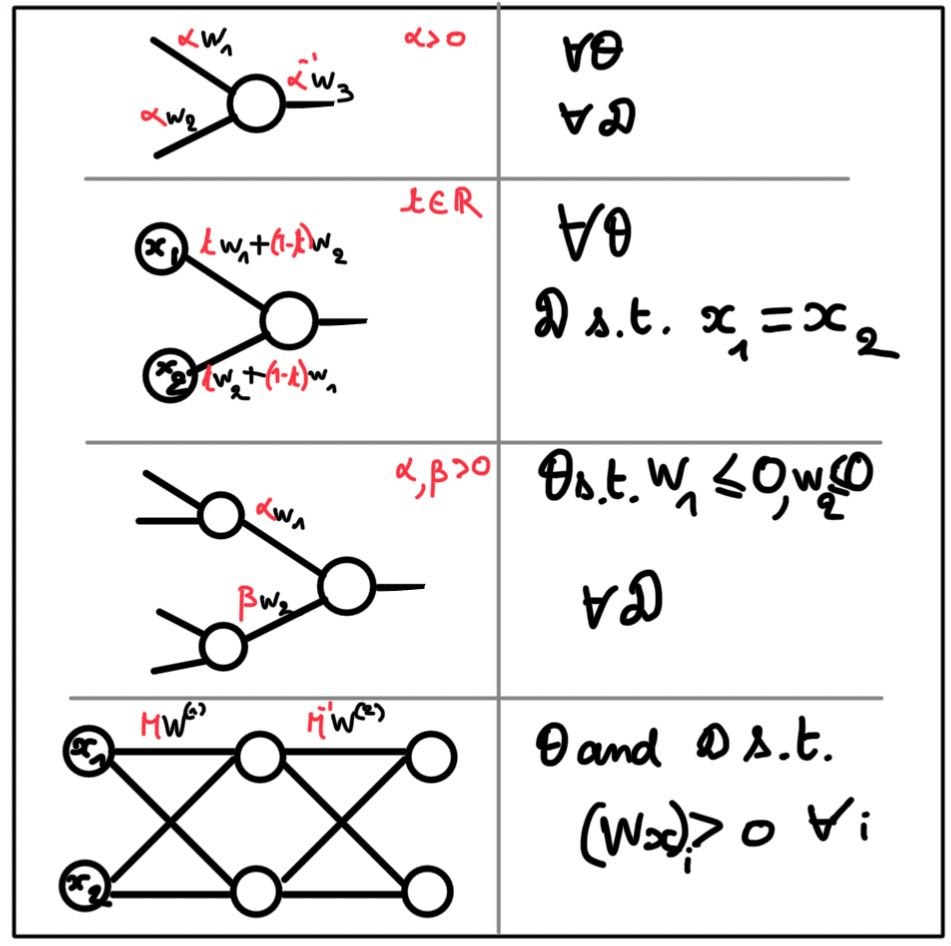
\includegraphics[width=0.33\linewidth]{images/draft/hierarchy-symmetries.jpg}
    \caption{From top to bottom:\textbf{(1.)} A rescaling symmetry is valid for all parameters and dataset. \textbf{(2.)} A shared input symmetry is valid at any neurons with equal inputs \textbf{(3.)} A dead ReLU symmetry is valid after layer $1$ for any neuron with all input parameter negative \textbf{(4.)} An active subspace symmetry is valid for parameter and data such that a set of neurons in a layer have positive only activations.\pnote{Last symmetry is harder to formalize: describe $M$}}
    \label{fig:hierarchy-symmetries}
\end{figure}

\myline

\paragraph{Data augmentation}
Data augmentation is a brute force approach in which a dataset is enriched with new samples crafted from original ones.
Note that a single continuous symmetry can generate infinitely many augmented points, so it is clear that the augmented dataset cannot be complete.
A drawback of data augmentation is the impact on storage and computational costs due to increase in data points.
In the symmetry discovery scenario, \cite{yang2023p4icml} reports better performances when using data augmentation generated from learned symmetries rather than pure equivariance to those learned symmetries even though for the ground truth symmetries, pure equivariance performs better.
Data augmentations may be the only game in town when the transformations are difficult to express with group theory (e.g. face recognition \cite{bhattacharya20192sicaccpi}), or to address example partial symmetry.
Instead of inferring symmetries as in symmetry discovery, some works propose to search directly for data augmentation policies with positive impact on the validation set \cite{cubuk20192iccvprc,lim2019anips}.
Data augmentation are often perceived as a cheap way to achieve invariance, less elegant than invariant architecture, but they have empirical success and are used frequently in industry.
\cite{shen2026} provides insight on the relevance of using equivariant architectures

\myline

\paragraph{Crafting invariant features}
Feature engineering, the goal is to featurize so that the featurization is invariant w.r.t. symmetries. However, this featurization might not be lossless, nor tailored to the specific need of the problem. Moreover one of the core strength of deep learning is learning representation, so doing featurization is doing by hand something that should be done by the model. 
\begin{itemize}
    \item random walk
    \item compute edge distances in geometric graphs
\end{itemize}

\myline

\paragraph{Predictable transformation}
Translate the input by one unit and rotate the output by a quarter. This is predictable but different from equivariance.
Or even in the case of scalar: move to the right by 1 unit and increase a scalar quantity by $C$ (constant) or move by 1 unit and multiply a quantity by $C$.

\myline

\paragraph{Interplay between invariance and equivariance in geometric deep learning}
A common scheme to build a globally invariant model is to stack equivariant layers and put an invariant layer at the end.

\myline

\paragraph{Symmetry to subsets of group, partial symmetry}
A relaxation discussed in \cite{romero2023} takes the form of achieving equivariance on a subset of a group (ex: rotations in [-90 degrees, +90 degrees] for face or on MNIST which has 6 and 9 potential confusion). This is particularly weird since the subset is not a group. This is also weird because a tilted 6 will not have the same range as a straight 6. \cite{romero2023} propose a way to have some layers fully equivariant and other layers partially equivariant.

\paragraph{Ranged symmetry} In this case, we would want to have symmetry over a specific range of transformations. For example for the MNIST dataset, we might ideally want symmetry to  some range of 2D rotations but not to the full 2D rotation group because otherwise digits 6 and 9 would be symmetries of each other. 

\paragraph{Small deformation} Consider a hand drawing. This drawing would still be recognizable even if it were drawn with some light tremors or instability. But if we apply the same "tremoring" operation again and again on the drawing, at some point it would not be considered the same anymore. This is another case of partial symmetry w.r.t. a transformation.

\myline

\paragraph{Derivative fields of geometric deep learning}
These derivative fields are less focused on symmetry.
\textit{Topological deep learning} is concerned with higher order message passing \cite{papillon2023,papamarkou2024}.
\textit{Categorical deep learning} seems to be concerned with programs and out of distribution generalization.

\myline

\paragraph{Geometric deep learning}
The objective of Geometric Deep Learning \cite{bronstein2017ispm, bronstein2021} is twofold: (1) provide a unifying view of deep learning architectures and (2) extend deep learning on new domains like graphs or manifolds in a convincing, principled way
In this field symmetry and equivariance are used a design principle.
This makes it possible to derive the form of a convolutional neural network from requiring translational equivariance, convolution is thus given a particular role.
\cite{kondor2018p3icml} argues that convolution is not just a way to achieve equivariance to a group action, it is also necessary necessary that an equivariant feedforward networks implements a (generalized group) convolution which takes the form 
\[
    (f\ast g)(u)=\int_Gf(uv^{-1})g(v)d\mu(v).
\]
The discrete counterpart of this equation for the correlation operation of functions having $K$ channels was introduced in \cite{cohen2016}, which reads by adapting notation to stay consistent with the above:
\[
    (f\star g)(u)=\sum_{v \in G}\sum_k^Kf_k(v)g_k(u^{-1}v).
\]
where $f$ and $g$ are functions on the group $G$.

\myline

\paragraph{Equivariant deep learning}
The field of equivariant deep learning can be seen as a subfield of Geometric Deep Learning focused on designing equivariant neural networks.
Diffusion models can be made equivariant: \cite{xu2026a} propose an architecture for molecular structure generation which constrains the target probability distribution to be SE(3)-equivariant.



\end{document}